\chapter[Projekt konstrukcji sonaru oraz protokoły komunikacji]{Projekt konstrukcji sonaru oraz protokoły komunikacji}

\label{chapter:konstrukcja}

% Tutaj powinien być opis części mechanicznej, schematy elektroniczne,
% opis protokołu komunikacji wraz z opisem implementacji (w protokole)
% listy poleceń.
% Opis funkcjonalności, które będą oferowane przez aplikację
% oraz sposob przetwarzania danych pomiarowych i ich reprezentacji.

\section{Komunikacja}

\subsection{Wybór protokołu}

Wybrany został protokół UART, ze wględu na to, że płytka deweloperska STM32 NUCLEO-L476RG 
z której skorzystano w projekcie posiada wbudowany konwerter UART$\rightarrow$~USB, 
co pozwala na skomunikowanie mikrokontrolera z komputerem bez dodatkowego sprzętu.

\subsection{Komputer \textrightarrow{} sonar}
Użytkownik systemu może wysłać z komputera instrukcję do wywołania całej sekwencji działania urządzenia. 
Ramka danych zaczyna się znakiem, który nie będzie nigdy występował  ułatwiającym rozpoznanie wiadomości, 
następnie musi zostać podany numer komendy informujący sonar jaką czynność powienien wykonać, 
parametry określające warunki tej czynności, a na koniec suma kontrolna wiadomości.

\begin{figure}[!ht] %data in
    \centering
    \begin{tikztimingtable}[timing/wscale=4]
        \tikzset{% Environment Config
            timing/dslope=0.1,
            timing/.style={x=5ex,y=2ex},
            x=5ex,
            timing/rowdist=3ex,
            timing/name/.style={font=\sffamily\scriptsize},
            timing/d/text/.style={font=\sffamily\tiny},
        }
        \textcolor{black}{Instruction} & [black]
            Z 1D{X}  1D{CMD\_ ID} 1D{PAR1} 1D{PAR2} 1D{PAR3}   1D{CRC}  \\ %
        \textcolor{black}{Bytes} & [black]
            Z 1D{1}  1D{1}        1D{1}    1D{1}    1D{4}      1D{4}    \\ %
        %
        % there must NOT be an uncommented line before \extracode!
        %
        \extracode
            \tablerules
        %%  \tablegrid
        
        \begin{pgfonlayer}{background}
            \begin{scope}[semitransparent ,semithick]
                %\vertlines[darkgray,dotted]{1.0,3.0,...,23.0}
                \vertlines[gray,dotted]{4.0,8.0,...,\twidth}
            \end{scope}
        \end{pgfonlayer}
        \end{tikztimingtable}
        \caption{Ramka danych przychodzących}
        \label{fig:datain}
    \end{figure}
    \todo{zrobić ładniejszą ramkę}

% \begin{figure}[!h]
%     \centering
%     \begin{tikztimingtable}[timing/wscale=4]
%         \tikzset{% Environment Config
%             timing/dslope=0.1,
%             timing/.style={x=5ex,y=2ex},
%             x=5ex,
%             timing/rowdist=3ex,
%             timing/name/.style={font=\sffamily\scriptsize},
%             timing/d/text/.style={font=\sffamily\tiny},
%         }
%         \busref*{FRAME}      & 2u 1d 2d 2u \\
%         \textcolor{black}{Instruction} & [black]
%             Z 1D{X}  1D{COM\_ID} 1D{CRC}    \\ %
%         \textcolor{black}{Bytes} & [black]
%             Z 1D{1}  1D{1}       1D{4}      \\ %
%         %
%         % there must NOT be an uncommented line before \extracode!
%         %
%         \extracode
%             \tablerules
%         %%  \tablegrid
        
%         \begin{pgfonlayer}{background}
%             \begin{scope}[semitransparent ,semithick]
%                 %\vertlines[darkgray,dotted]{1.0,3.0,...,23.0}
%                 \vertlines[gray,dotted]{4.0,8.0,...,\twidth}
%             \end{scope}
%         \end{pgfonlayer}
%         \end{tikztimingtable}
%     \end{figure}
    

\subsection{Sonar \textrightarrow{} komputer}

Sonar w odpowiedzi na instrukcję wysyła ramkę danych która również zaczyna się znakiem specjalnym, 
następnie podawany jest numer komendy na którą sonar odpowiada, status wykonania, dane pomiarowe oraz suma kontrolna.
\begin{figure}[!ht] %data out
\centering
\begin{tikztimingtable}[timing/wscale=4]
    \tikzset{% Environment Config
        timing/dslope=0.1,
        timing/.style={x=5ex,y=2ex},
        x=5ex,
        timing/rowdist=3ex,
        timing/name/.style={font=\sffamily\scriptsize},
        timing/d/text/.style={font=\sffamily\tiny},
    }
    \textcolor{black}{Instruction} & [black]
        Z 1D{X}  1D{ANS\_ID} 1D{STATUS} 1D{ZC\_NUM} 1D{TCL} 1D{D11} 1D{...} 1D{D33}  1D{CRC}  \\ %
    \textcolor{black}{Bytes} & [black]
        Z 1D{1}  1D{1}       1D{1}      1D{1}       1D{4}   1D{4}   1D{...} 1D{4}    1D{4}    \\ %
    %
    % there must NOT be an uncommented line before \extracode!
    %
    \extracode
        \tablerules
    %%  \tablegrid
    
    \begin{pgfonlayer}{background}
        \begin{scope}[semitransparent ,semithick]
            %\vertlines[darkgray,dotted]{1.0,3.0,...,23.0}
            \vertlines[gray,dotted]{4.0,8.0,...,\twidth}
        \end{scope}
    \end{pgfonlayer}
    \end{tikztimingtable}
    \caption{Ramka danych wychodzących}
    \label{fig:dataout}
\end{figure}
\todo{zrobić ładniejszą ramkę}


\section{Konstrukcja układów elektronicznych sonaru}
Projekt bazuje na autorskiej płytce z obwodem drukowanym, który został zaprojektowany przy pomocy 
otwartoźródłowego narzędzia do projektowania elektroniki ,,KiCad" \cite{kicad}. 
Całe urządzenie składa się z płytki deweloperskiej oraz zaprojektowanego na cele pracy dyplomowej 
PCB\footnote[1]{Printed Circuit Board}, które
jest podłączone do Nucleo w formie ,,shieldu"\todo{pokazać jak wygląda shield} poprzez listwy kołkowe.
Całą elektronikę można podzielić na kilka bloków, które spełniają określone fukcje, 
jest to międzyinnymi sekcja zasilania, część nadawcza, część odbiorcza, zestaw filtrów sygnału przychodzącego oraz komparatory progujące sygnał.
\todo{wstawić diagram funkcjonalny}

\subsection{Zasilanie}
Całe urządzenie zasilane jest z portu USB komputera, które jednocześnie służy do komunikacji. 
Przewód jest podłączony bezpośrednio do płytki deweloperskiej Nucleo, gdyż posiada ona już wbudowane złącze. 
Mimo, że płytka deweloperska posiada wyprowadzenia zarówno \unit[5]{V} jak i \unit[3,3]{V}, 
postanowiłem zaimplementować układ stabilizatora liniowego obniżajcego napięcie do \unit[3,3]{V} w celu lepszej izolacji zasilania układów analogowych od cyfrowych co powinno przełożyć się na mniejsze zakłócenia.
\begin{figure}[ht!]
    \centering
    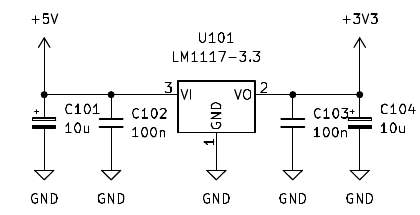
\includegraphics[width = 0.5\textwidth]{LDO.png}
    \caption{Stabilizator napięcia}
    \label{fig:ldo}
\end{figure}

\subsection{Nadajnik}
Rolę nadajnika pełni przetwornik piezoelektryczny o średnicy \unit[16]{mm} i częstotliwości rezonansowej \unit[40]{kHz},\todo{dodać model przetwornika} która to jest poza spektrum słyszalnych częstotliwości.
\begin{figure}[ht!]
    \centering
    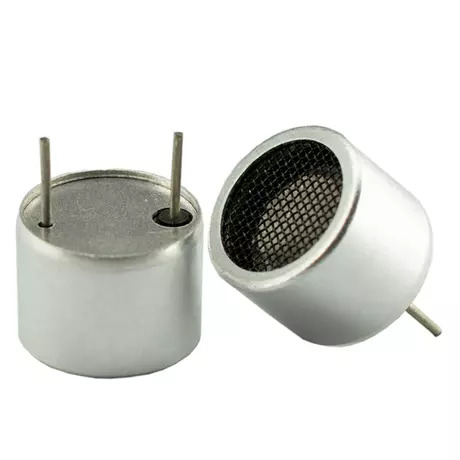
\includegraphics[width = 0.3\textwidth]{piezo.jpeg}
    \caption{Nadajnik piezoelektryczny}
    \label{fig:piezo}
\end{figure}
\todo{dodać źródło}

\subsection{Wzmacniacz nadajnika}
W celu uzyskania mocnego sygnału ultradźwiękowego z przetwornika piezoelektrycznego zaprojektowano układ wzmacniający z transformatorem. 
Synał nadający częstotliwość wysyłany jest z mikroprocesora, następnie jest wzmacniany parą tranzystorów, razem tworzących układ Darlingtona, 
który zapewnia duże wzmocnienie prądowe sygnału i zachowuje krótkie czasy przełączania charakterystyczne dla tranzystorów bipolarnych.
Transformator w tym układzie służy do podniesienia napięcia które trafia na przetwornik, docelowo jest to nawet szczytowo \unit[80]{V} co sprawia, 
że sygnał jest bardzo mocny.
\todo{akapity}
Układ posiada również zabezpieczenie przed zbyt długim czasem otwarcia tranzystora, sygnał jest przepuszczany przez kondensator, 
co sprawia, że tylko szybkozmienne przebiegi są w stanie dotrzeć na bazę klucza. 
Zbyt długa ekspozycja transformatora na przepływ prądu mogłaby go narazić na przegrzanie.
Ze względu na indukcyjny charakter uzwojeń transformatora podczas szybkiej zmiany generowanego pola magnetycznego następuje 
konwersja tej energii do postaci prądu zwrotnego wyindukowanego na tej cewce, aby uchronić się przed niepożądanym działaniem tego zjawiska, 
równolegle z uzwojeniem pierwotnym sprzężona jest dioda Schottkiego, która pozwala zniwelować ten prąd.
Dodatkowo jako element ułatwiajacy pracę nad urządzeniem, dodany został LED, który emituje światło w trakcie przepływu prądu przez transformator.
\begin{figure}[ht!]
    \centering
    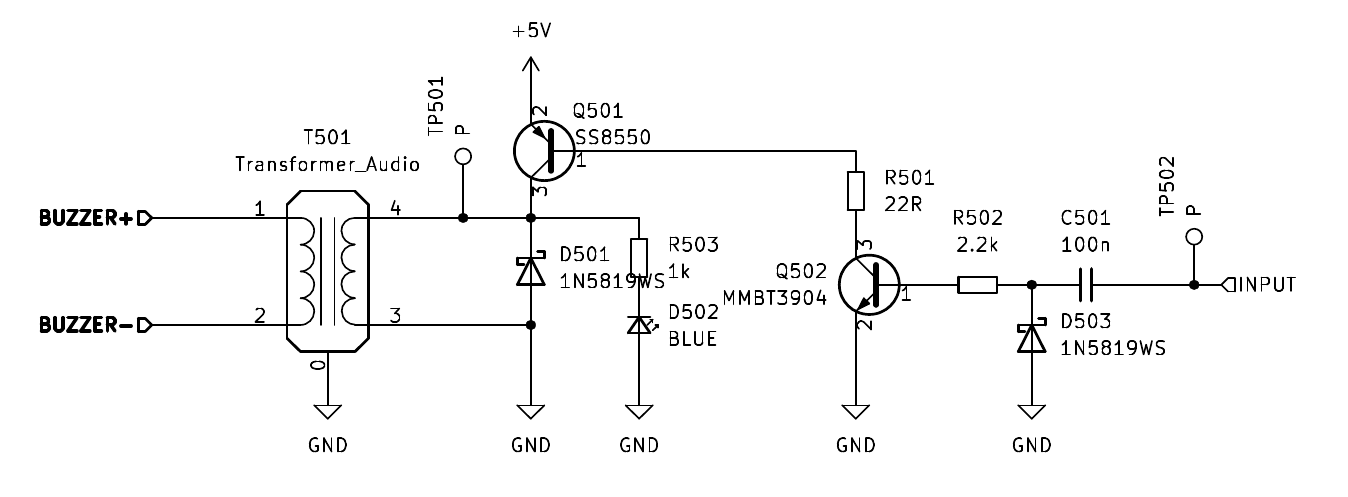
\includegraphics[width = 0.7\textwidth]{piezo_amp.png}
    \caption{Wzmacniacz sygnału nadajnika piezoelektrycznego}
    \label{fig:piezo_amp}
\end{figure}

\subsection{Filtry sygnału audio}

Rolę odbiorników będą pełnić trzy dookólne mikrofony MEMS, które cechują się względnie liniową charakterystyką przenoszenia pasma. 
Dlatego też konieczne będzie zastosowanie dla każdego z nich zestawu filtrów pasmowych, które przepuszczą nam tylko i wyłącznie częstotliwości bliskie częstotliwości 
sygnału jaki generuje przetwornik piezoelektryczny, a zablokują wszytskie nieporządane. 
Pojedynczy stopień filtra, dawałby na wyjściu zbyt niski zakres poziomu napięć, 
z tego powodu sygnał przechodzi przez 3 stopnie wzmacniaczy operacyjnych. Takie rozwiązanie zarówno filtruje sygnał i wzmacnia go.
\begin{figure}[ht!]
    \centering
    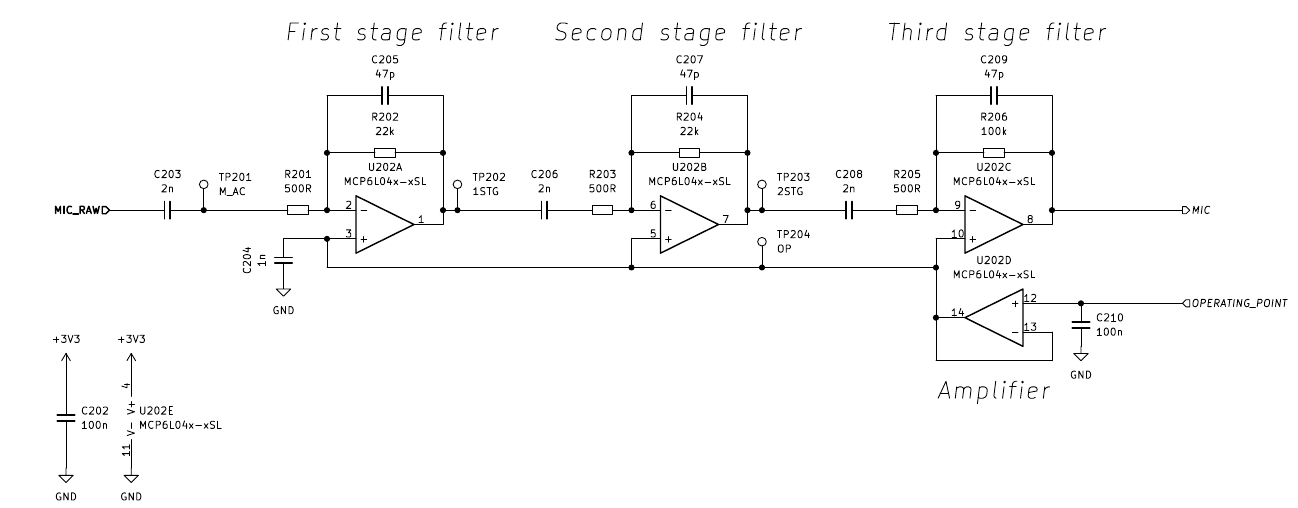
\includegraphics[width = \textwidth]{filter.png}
    \caption{Zestaw filtrów dla sygnału z mikrofonów}
    \label{fig:filter}
\end{figure}

\todo{opisać obszernie wybór wzmacniaczy operacyjnych}

Zazwyczaj układy analogowe oparte o wzmacniacze operacyjne zasilane są napięciem symetrycznym a sygnał przemienny oscyluje wokół potencjału masy. 
W tym wypadku ze względu na zakres napięciowy wejść mikroprocesora do zasilania wzmacniaczy uperacyjnych 
zostało użyte pojedyncze napięcie \unit[3,3]{V} zamiast symetrycznego co oznacza, 
że chcąc uzyskać napięcie odniesienia w połowie zakresu zasilania należy ustalić je na poziomie \unit[1,65]{V}. 
Tę wartość ustala dzielnik napięcia z dwóch identycznych rezostorów,
a wzmacniacz operacyjny zwiększa wydajność prądową takiego źródła. 
\begin{figure}[ht!]
    \centering
    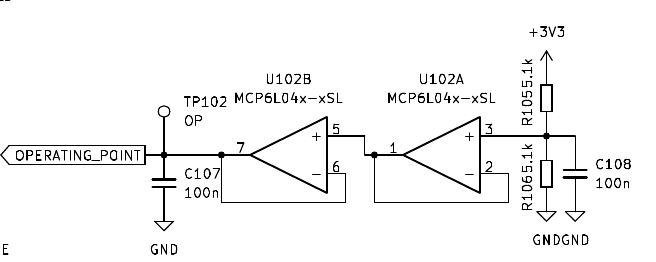
\includegraphics[width=0.5\textwidth]{op_point.png}
    \caption{Wzmacniacz prądowy napięcia odniesienia}
    \label{fig:op_point}
\end{figure}

\subsection{Progowanie sygnału}
Wejścia licznika reagują na zbocza sygnału cyfrowego, co oznacza, że analogowy sygnał z wyjścia filtra musi zostać przetworzony na stany logiczne.
Dokładna wartość napięcia nie jest potrzebna. Istotne są punkty przecięcia się sinusoidy z osią przebiegu.
Takie zadanie idealnie spełnia komparator \ref*{fig:comparator}, próg od którego sygnał ma interpretować jako wysoki stan jest podawany w formie 
napęcia z przetowrnika DAC mikrokontrolera dodatkowo wzmocnionego wzmacniaczem operacyjnym \ref*{fig:thereshold}.
Pozwala to na reagowanie tylko na falę dźwiękową o wystarczająco dużej amplitudzie, 
a po wykryciu mocnego sygnału wrócić z powrotem do poziomu napięcia odniesienia sygnału gdzie pomiar jest najdokładniejszy.

\begin{figure}[ht!]
    \centering
    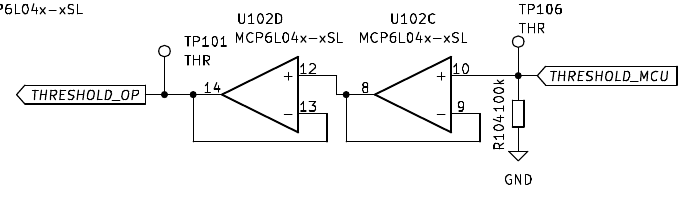
\includegraphics[width=0.5\textwidth]{thereshold.png}
    \caption{Wzmacniacz wartości progowej}
    \label{fig:thereshold}
\end{figure}

\begin{figure}[ht!]
    \centering
    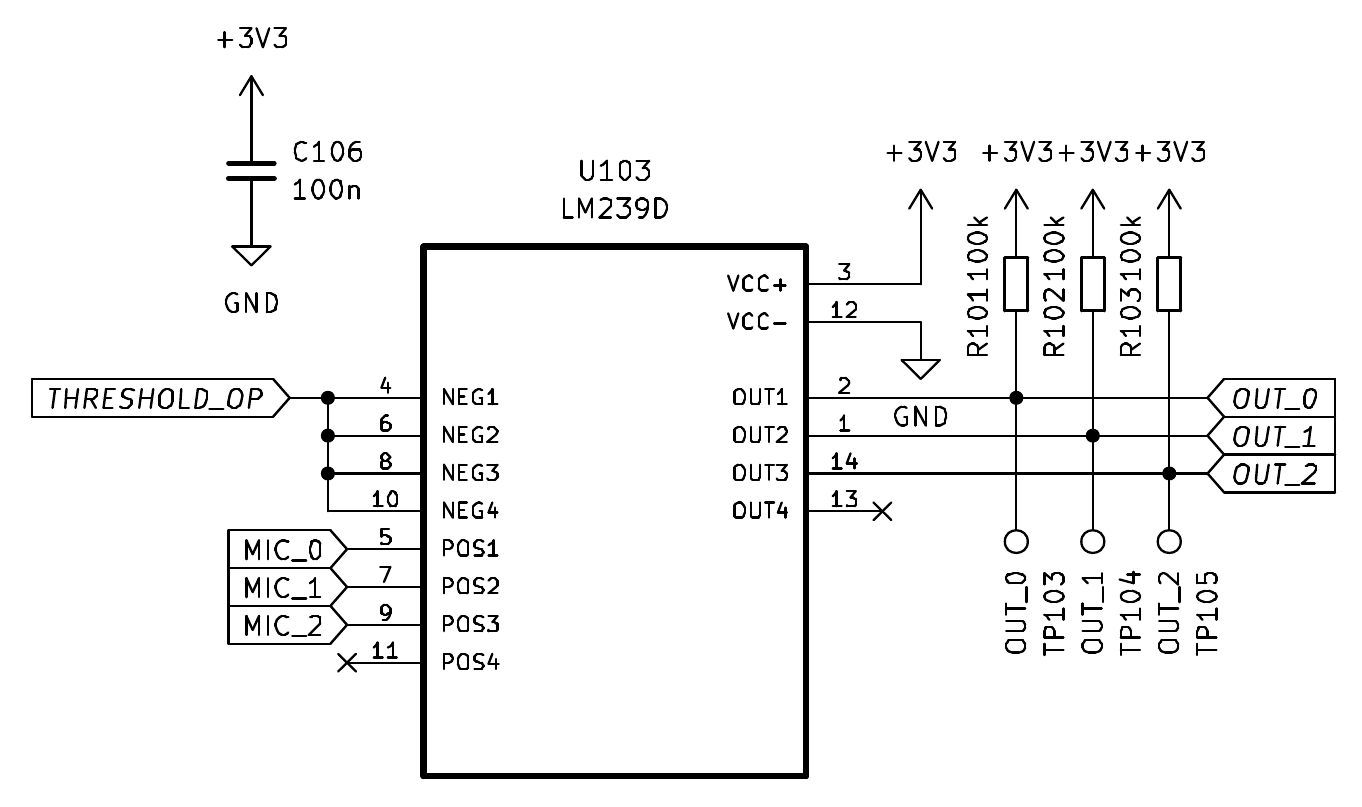
\includegraphics[width=0.5\textwidth]{comparator.png}
    \caption{Czterokanałowy komparator}
    \label{fig:comparator}
\end{figure}

\section{Konfiguracja mikrokontrolera}

\begin{figure}[ht!]
    \centering
    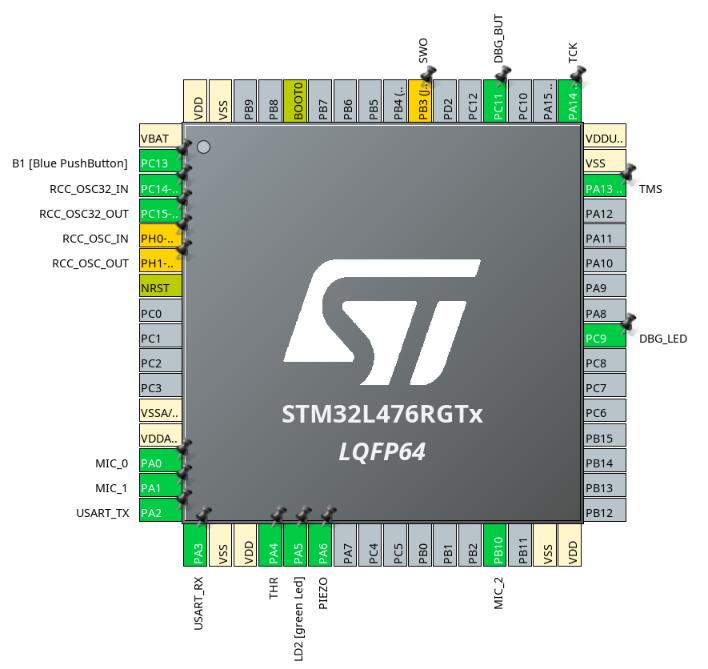
\includegraphics[width=0.5\textwidth]{cube.png}
    \caption{Konfiguracja pinów mikrokontrolera}
    \label{fig:cube}
\end{figure}

\begin{figure}[ht!]
    \centering
    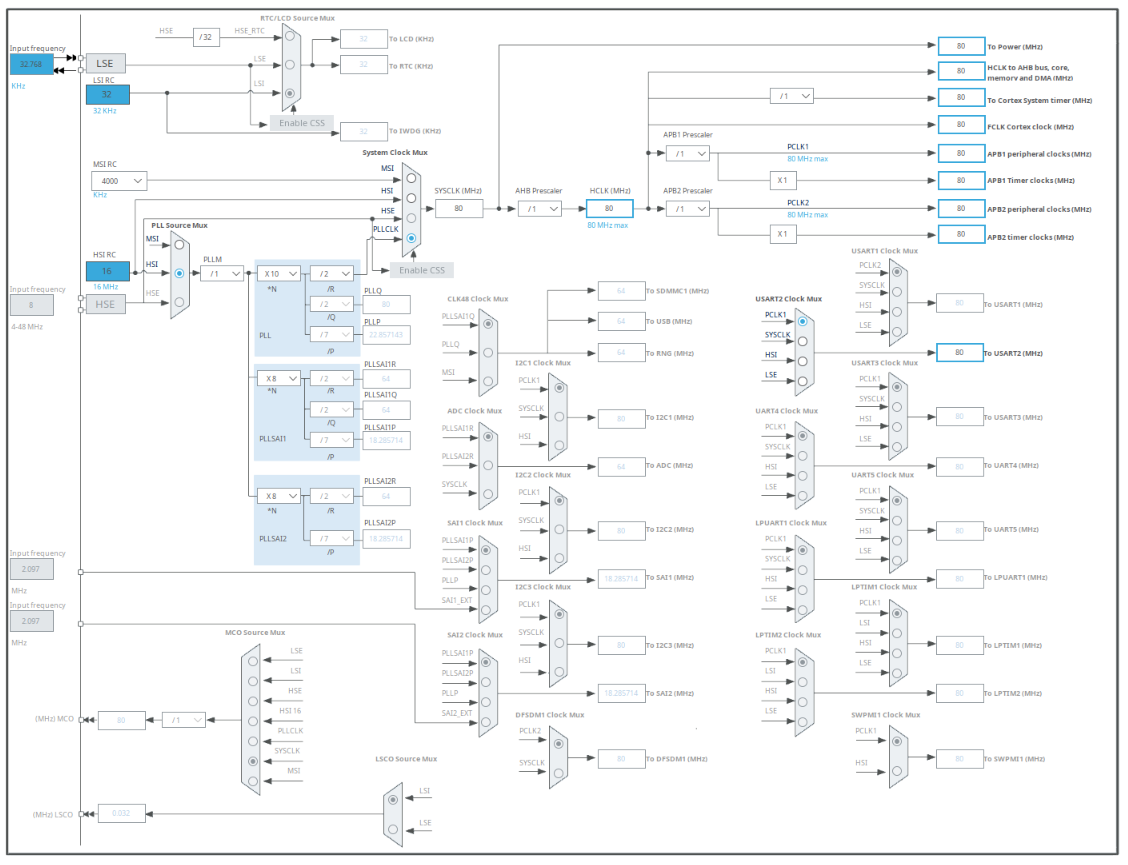
\includegraphics[width=\textwidth]{cube_clocks.png}
    \caption{Konfiguracja zegarów mikrokontrolera}
    \label{fig:cube_clocks}
\end{figure}



